\documentclass[11pt]{article}
\usepackage[margin=1.1in]{geometry}
\usepackage{amsmath,amssymb,amsthm}
\usepackage{graphicx}
\usepackage{booktabs}
\usepackage[numbers,sort&compress]{natbib}
\usepackage{xcolor}
\definecolor{linkblue}{rgb}{0,0,0.55}
\usepackage[colorlinks=true,linkcolor=linkblue,citecolor=linkblue,urlcolor=linkblue]{hyperref}
\usepackage{microtype}
\usepackage{enumitem}

\makeatletter
\renewcommand\paragraph{\@startsection{paragraph}{4}{\z@}%
  {3.25ex \@plus1ex \@minus.2ex}{-1em}%
  {\normalfont\normalsize\itshape}}
\makeatother

\newtheorem{theorem}{Theorem}[section]
\newtheorem{proposition}[theorem]{Proposition}
\newtheorem{lemma}[theorem]{Lemma}
\newtheorem{corollary}[theorem]{Corollary}
\theoremstyle{definition}
\newtheorem{definition}[theorem]{Definition}
\newtheorem{assumption}[theorem]{Assumption}
\theoremstyle{remark}
\newtheorem{remark}[theorem]{Remark}
\newtheorem{example}[theorem]{Example}

\newcommand{\R}{\mathbb{R}}
\newcommand{\E}{\mathbb{E}}
\newcommand{\ip}[2]{\langle #1,#2\rangle}
\newcommand{\lc}{\ell}
\newcommand{\lcs}{\ell^{*}}
\newcommand{\ST}{\operatorname{ST}}
\newcommand{\dom}{\operatorname{dom}}
\newcommand{\sgn}{\operatorname{sgn}}
\newcommand{\artanh}{\operatorname{artanh}}
\newcommand{\sech}{\operatorname{sech}}
\newcommand{\diag}{\operatorname{diag}}
\newcommand{\inter}{\operatorname{int}}
\newcommand{\zono}{\mathcal{Z}}
\DeclareMathOperator*{\argmax}{arg\,max}
\DeclareMathOperator*{\argmin}{arg\,min}

\title{Bounded Market Makers from Convex Duality:\\
Self-Set Fees, Dead Bands, and the Order Book as a Theorem}
\author{Peter Cotton\\ Microprediction\\ \texttt{peter.cotton@microprediction.com}}
\date{Working draft v0.1 \textperiodcentered{} October 2026}

\begin{document}
\maketitle

\begin{abstract}
We study automated market makers for contracts that settle to bounded real payoffs, such as a saturated surprise
relative to a published forecast, rather than to the indicator of an outcome. The cost function
$C(q)=b\sum_{d}\log\cosh(\ip{q}{v_d}/b)$, built from \emph{residual directions} $v_d$ supplied by the market maker
and its capital $b>0$, has a convex conjugate that is finite exactly on the zonotope $V[-1,1]^{D}$. The worst-case
loss is therefore exactly $b\,D\log 2$, the price set is the interior of the zonotope, and the Hessian is a
covariance quoted by vectors, revealed through cross-impact and depleted by inventory. Any cost that is a state
function refunds itself over a round trip, so revenue must be path-dependent, and a per-unit fee $f\|\delta\|_1$
set by each maker is a \emph{dead band} in price space: a trader with belief $\pi$ transacts nothing exactly when
$\pi\in p(q)+[-f,f]^{n}$, and otherwise solves a lasso whose solution is sparse across contracts. Aggregating
fee-bearing makers is an inf-convolution whose supply is the horizontal sum of band-limited supplies, so a
consolidated limit order book, with a level at each maker's quote, depth equal to its curvature and exact zero
fills for uncompetitive makers, follows as a theorem.
\end{abstract}

\section{Introduction}

A cost-function market maker \citep{hanson2003,hanson2007,chen2007utility,abernethy2013} quotes a price vector
$p(q)=\nabla C(q)$ for a convex potential $C$ of its net position $q$, and charges a trader who moves the position
from $q$ to $q+\delta$ the amount $C(q+\delta)-C(q)$. The logarithmic market scoring rule (LMSR) is the case
$C(q)=b\log\sum_i e^{q_i/b}$ on a complete set of mutually exclusive outcomes, and its celebrated properties all follow from the
convex-analytic structure of $C$ \citep{abernethy2013}: prices that are probabilities, a worst-case loss of
$b\log n$, and an interpretation as a sequentially shared proper scoring rule.

We work out the same programme for the setting that arises when a market is attached to a \emph{forecast}:
contracts that settle to a bounded, real-valued \emph{surprise} relative to a
published baseline rather than to the indicator of an outcome. Three design pressures shape the construction.

\begin{enumerate}[leftmargin=2em]
\item \textbf{Bounded loss must be exact, not asymptotic.} A market maker that posts capital $b$ should be able to
state its worst-case loss in closed form, and the bound should be attained at a nameable settlement. We obtain
$b\,D\log 2$ for $D$ quoted directions, attained at vertices of a zonotope (Theorem~\ref{thm:loss}).

\item \textbf{Correlation must be quoted cheaply and truthfully.} A market maker across $n$ related contracts has a
view about their joint behaviour. Asking for an $n\times n$ covariance matrix is both expensive and unreliable in
practice (it is never positive semidefinite after editing). We ask instead for residual \emph{vectors}; their Gram
matrix is automatically PSD, and it is exactly the Hessian of $C$ at the origin (Section~\ref{sec:curvature}). The
cross-impact traders observe is therefore the covariance the maker is prepared to accept fills under.

\item \textbf{The protocol should fix as little as possible.} Fees are not a parameter of the mechanism but a quote
of each maker; aggregation across makers should need no auction, no central book and no parameter. We show that
with fee-bearing costs, convex duality alone produces the consolidated limit order book (Theorem~\ref{thm:book}).
\end{enumerate}

The last point inverts the usual relationship between automated market makers and order books. Order books are typically presented as the primitive and automated makers as an approximation to
them; here a book with discrete levels and finite depth is the \emph{aggregate} of smooth makers, and the discreteness
comes entirely from the fee.

The mathematics is elementary (inf-convolution, conjugacy and soft thresholding) and has a textbook economic
reading: price is marginal cost, aggregation is Marshall's horizontal summation of supply
curves, the conjugate is Hotelling's profit function. The two departures from producer theory are that production
here is reversible, which is why the fee must be added by hand, and that the firm is a multiproduct one with
economies of scope made tractable by compression of its cost structure into a few residual directions.

\paragraph{Contributions.} (i) The bounded cost family and its conjugate in closed form, with an exact and attained
loss bound and an exact description of the price set (Section~\ref{sec:bounded}). (ii) The fee as the unique
path-dependent charge and as a dead band; the trader's problem as a lasso with exact sparsity
(Section~\ref{sec:fees}). (iii) The aggregation theorem: the conjugate of the inf-convolution is the sum of the
conjugates; the aggregate supply is the horizontal sum of band-limited supplies; the limit order book, the
additivity of liquidity near the origin and the one-dimensional routing problem (Section~\ref{sec:aggregation}).
(iv) The curvature structure: covariance quoted by vectors, revealed by cross-impact, depleted by inventory, and a
conservation law for curvature and collateral (Section~\ref{sec:curvature}). (v) The duality with proper scoring
rules and follow-the-regularised-leader, and the fee as a regularisation parameter (Section~\ref{sec:duality}).
(vi) Numerical verification of every statement (Section~\ref{sec:numerics} and Appendix~\ref{app:verify}).

\section{Setting}\label{sec:setting}

There are $n$ contracts. Contract $i$ settles to a real number $s_i\in[-1,1]$. In the application that motivates
us, $s_i=\tanh(z_i/\kappa)$ where $z_i$ is a standardised surprise, the realised value of a quantity minus a frozen
baseline forecast, in units of the baseline's own standard deviation. The saturating transform is deliberate: it
bounds payouts, makes the influence of a single corrupt observation bounded, guarantees that all moments exist, and
makes the price a bounded quantity, the market's expected correction to the baseline. Nothing
below depends on the choice of $\tanh$; only $s\in\mathcal{S}\subseteq[-1,1]^{n}$ is used.

A market maker holds a net position $q\in\R^{n}$: $q_i$ is the number of units of contract $i$ it has sold. It
quotes through a convex, differentiable cost function $C:\R^{n}\to\R$ with $C(0)=0$. A trader who buys the bundle
$\delta\in\R^{n}$ pays $C(q+\delta)-C(q)$, and the instantaneous price is $p(q)=\nabla C(q)$. At settlement the
maker pays $\ip{q}{s}$. Starting from $q=0$, the maker's realised profit after a sequence of trades totalling $q$ is
$C(q)-\ip{q}{s}$; it does not depend on the path, only on $q$. We write $C^{*}(s)=\sup_{q}\{\ip{q}{s}-C(q)\}$ for
the convex conjugate, so that the maker's worst-case loss against settlement $s$ is exactly $C^{*}(s)$.

\section{The bounded cost family}\label{sec:bounded}

\begin{definition}[Residual directions and capital]
Let $V=[v_1\;\cdots\;v_D]\in\R^{n\times D}$ have full row rank, let $b>0$, and let $\lc(x)=\log\cosh x$. The
\emph{bounded market maker} with directions $V$ and capital $b$ has cost
\begin{equation}\label{eq:cost}
C_{b,V}(q)=b\sum_{d=1}^{D}\lc\!\left(\frac{\ip{q}{v_d}}{b}\right)=b\,\mathbf 1^{\top}\lc\!\left(V^{\top}q/b\right),
\end{equation}
price $p(q)=\nabla C_{b,V}(q)=V\tanh(V^{\top}q/b)$, and Hessian
\begin{equation}\label{eq:hess}
H(q)=\nabla^{2}C_{b,V}(q)=\tfrac1b\,V\diag\!\big(\sech^{2}(V^{\top}q/b)\big)V^{\top}.
\end{equation}
\end{definition}

The function $\lc$ is even, convex, $\lc(0)=\lc'(0)=0$, $\lc''(x)=\sech^2 x\le 1$, and $\lc(x)=|x|-\log 2+o(1)$ as
$|x|\to\infty$. Its conjugate is the binary-entropy-like function
\begin{equation}\label{eq:lcs}
\lcs(y)=\sup_x\{xy-\lc(x)\}=
\begin{cases}
\tfrac12\big[(1+y)\log(1+y)+(1-y)\log(1-y)\big], & |y|\le 1,\\
+\infty, & |y|>1,
\end{cases}
\end{equation}
with $\lcs(0)=0$, $\lcs(\pm1)=\log 2$, $(\lcs)'(y)=\artanh y$, and $0\le\lcs\le\log 2$ on $[-1,1]$.

\begin{lemma}[Conjugate]\label{lem:conj}
Let $\zono_V=V[-1,1]^{D}=\{Vy:\|y\|_\infty\le1\}$ be the zonotope generated by the columns of $V$. Then
\begin{equation}\label{eq:conj}
C_{b,V}^{*}(s)=\min\Big\{\,b\sum_{d=1}^{D}\lcs(y_d)\;:\;Vy=s,\ \|y\|_\infty\le 1\Big\}
\quad\text{for }s\in\zono_V,
\end{equation}
and $C_{b,V}^{*}(s)=+\infty$ for $s\notin\zono_V$. In particular $0\le C_{b,V}^{*}\le b\,D\log 2$ on $\zono_V$,
with $C^{*}_{b,V}(s)=b\,D\log2$ whenever $s=Vy$ for a vertex $y\in\{-1,1\}^D$ with no other representation in
$[-1,1]^{D}$.
\end{lemma}

\begin{proof}
Write $C_{b,V}=g\circ V^{\top}$ with $g(z)=b\sum_d\lc(z_d/b)$, a finite convex function on $\R^{D}$ with
$g^{*}(y)=b\sum_d\lcs(y_d)$. Since $g$ is finite everywhere and $V^{\top}$ is linear, \citet[Thm.\ 16.3]{rockafellar1970}
gives $(g\circ V^{\top})^{*}(s)=\inf\{g^{*}(y):Vy=s\}$ and the infimum is attained when finite. $\dom g^{*}=[-1,1]^{D}$,
so the conjugate is finite exactly on $V[-1,1]^{D}$. The bounds follow from $0\le\lcs\le\log2$ on $[-1,1]$, and the
vertex statement from the uniqueness of the representation.
\end{proof}

\begin{theorem}[Exact worst-case loss]\label{thm:loss}
Let the settlement set satisfy $\mathcal{S}\subseteq\zono_V$. Then for every trading history the loss of the bounded
market maker is at most $\sup_{s\in\mathcal{S}}C_{b,V}^{*}(s)\le b\,D\log 2$, and the bound $b\,D\log2$ is attained:
if $s=Vy$ with $y\in\{-1,1\}^{D}$ a uniquely represented vertex, the trader bundle $q_t=t\,V^{-\top}y$ with
$t\to\infty$ (when $D=n$, so that every $y$ is uniquely represented) drives the loss to $b\,D\log2$. If $\mathcal{S}\not\subseteq\zono_V$ the worst-case
loss is infinite.
\end{theorem}

\begin{proof}
The maker's loss against $s$ after trades totalling $q$ is $\ip{q}{s}-C(q)\le C^{*}(s)$, with the supremum over $q$
equal to $C^{*}(s)$ by definition; apply Lemma~\ref{lem:conj}. For attainment, $V^{\top}q_t=ty$, so
$\ip{q_t}{s}-C(q_t)=t\|y\|^2-b\sum_d\lc(t/b)\to b\,D\log 2$ since $\|y\|^2=D$ and $t-b\lc(t/b)\to b\log2$. If some
$s\in\mathcal{S}$ lies outside $\zono_V$ then $C^{*}(s)=+\infty$ and the supremum over $q$ is unbounded.
\end{proof}

\begin{corollary}[Defaults guarantee the bound]\label{cor:defaults}
If $V$ contains the scaled coordinate directions $m_ie_i$ with $m_i\ge1$ for every $i$ (the maker always quotes at
least the baseline's own marginals, possibly inflated by a volatility multiplier) then $[-1,1]^{n}\subseteq\zono_V$,
so every settlement in $[-1,1]^{n}$ is covered and Theorem~\ref{thm:loss} applies with $D\ge n$. Adding further
residual directions only enlarges $\zono_V$ and raises the bound by $b\log2$ per direction.
\end{corollary}

\begin{proposition}[The price set]\label{prop:priceset}
$p(\R^{n})\subseteq\inter\zono_V$. If $D=n$ (so $V$ is invertible) then $p(\R^{n})=\inter\zono_V=V(-1,1)^{n}$, and
$p$ is a diffeomorphism of $\R^{n}$ onto it with inverse $q(p)=b\,V^{-\top}\artanh(V^{-1}p)$.
\end{proposition}

\begin{proof}
$p(q)=V\tanh(V^{\top}q/b)$ and $\tanh$ maps $\R^{D}$ into $(-1,1)^{D}$, whose image under $V$ is $\inter\zono_V$
when $V$ has full row rank. When $D=n$, $V^{\top}q$ ranges over all of $\R^{n}$ and $\tanh$ is a bijection onto
$(-1,1)^{n}$; the inverse formula is immediate.
\end{proof}

Proposition~\ref{prop:priceset} is the analogue of ``LMSR prices are probabilities'': prices lie in the convex hull of
the settlement set, so no portfolio has a riskless profit against the maker, and the maker never quotes a price it
could not be settled at. The zonotope replaces the simplex because settlements are bounded reals rather than
indicators of exhaustive outcomes.

\begin{example}[One contract]\label{ex:one}
With $n=D=1$, $v=1$: $C(q)=b\log\cosh(q/b)$, $p(q)=\tanh(q/b)$, $q(p)=b\artanh p$, $C^{*}(s)=b\lcs(s)$, worst-case
loss $b\log2$ at $s=\pm1$. The loss $|q|-C(q)$ as a function of the position is increasing and saturates at
$b\log2$; the price saturates at $\pm1$; the depth $1/p'(q)=b\cosh^{2}(q/b)$ grows without bound as the maker's
inventory grows, so the maker charges more and more per unit as it approaches its loss bound, and would require an
infinite payment to move its price to $\pm1$. Compare the quadratic cost $q^2/2b$, which is Gaussian at the core
but has unbounded loss, and the LMSR, which is bounded but whose price moves with the same curvature at every
inventory level. The log-cosh maker is Gaussian at the core and bounded at the edges.
\end{example}

\section{Fees and the dead band}\label{sec:fees}

\paragraph{State functions refund themselves.} For any cost $C$, a round trip $q\to q+\delta\to q$ costs the trader
$[C(q+\delta)-C(q)]+[C(q)-C(q+\delta)]=0$. This is not a defect of a particular $C$ but of the class: a charge that
is a state function along every path integrates to zero around every closed loop. Curvature therefore cannot be a
source of revenue; it is an inventory-control device. The market maker's revenue, and its only defence against a
trader who repeatedly round-trips to extract information or liquidity, must be path-dependent.

\begin{definition}[Fee-bearing cost]
Fix a fee $f\in\R^{n}_{\ge0}$ (per unit, per contract). At state $q$ the trader buying $\delta$ pays
\begin{equation}\label{eq:feecost}
C^{f}_{q}(\delta)=C(q+\delta)-C(q)+\ip{f}{|\delta|},
\end{equation}
where $|\delta|$ is componentwise. A round trip of size $\delta$ now costs $2\ip{f}{|\delta|}>0$.
\end{definition}

Among charges that are positively homogeneous of degree one in $\delta$, continuous, and depend on $\delta$ alone,
the weighted $\ell_1$ norm is the natural one: it is the support function of the box $[-f,f]^n$, so it is the
cheapest path-dependent charge whose conjugate is an indicator, and that is exactly what makes the fee a dead band.

\begin{proposition}[The fee is a dead band in price space]\label{prop:band}
Let a trader hold a belief $\pi\in\R^{n}$ about the settlement mean and choose $\delta$ to maximise
$\ip{\delta}{\pi}-C^{f}_{q}(\delta)$. Then
\begin{enumerate}[leftmargin=2em,itemsep=0pt]
\item $\delta=0$ is optimal if and only if $\pi\in p(q)+[-f,f]^{n}$, i.e.\ $|\pi_i-p_i(q)|\le f_i$ for every $i$.
Thus the maker's bid and ask for contract $i$ are $p_i(q)\mp f_i$, and the bid--ask spread is $2f_i$.
\item At an optimum, for every $i$ with $\delta_i\ne0$, $\ p_i(q+\delta)=\pi_i-f_i\sgn\delta_i$, and for every $i$
with $\delta_i=0$, $\ |\pi_i-p_i(q+\delta)|\le f_i$.
\item The conjugate of the fee-bearing cost is an inf-convolution:
$(C^{f}_{q})^{*}(\pi)=\inf_{\|u\|_\infty\le f}\big\{C^{*}(\pi-u)-\ip{q}{\pi-u}+C(q)\big\}$, the $\ell_\infty$-ball
of radius $f$ smearing the conjugate of the fee-free cost. When $C(q)=\sum_iC_i(q_i)$ is separable, the optimal trade moves each price to the
soft-thresholded belief, $p_i(q+\delta)=p_i(q)+\ST_{f_i}\big(\pi_i-p_i(q)\big)$ with $\ST_f(x)=\sgn(x)\max(|x|-f,0)$.
\end{enumerate}
\end{proposition}

\begin{proof}
The objective is concave in $\delta$; $0$ is optimal iff $\pi\in\partial C^{f}_{q}(0)=\nabla C(q)+\partial\ip{f}{|\cdot|}(0)
=p(q)+[-f,f]^{n}$. Item 2 is the subgradient condition $\pi\in\nabla C(q+\delta)+f\odot\partial|\delta|$. Item 3 is
the conjugate of a sum, $(A+B)^{*}=A^{*}\,\square\,B^{*}$ \citep[Thm.\ 16.4]{rockafellar1970}, with $B=\ip{f}{|\cdot|}$
whose conjugate is the indicator of $\|\cdot\|_\infty\le f$ componentwise, and $A(\delta)=C(q+\delta)-C(q)$ whose
conjugate is $C^{*}(\cdot)-\ip{q}{\cdot}+C(q)$. In the separable case item 2 reads $p_i(q_i+\delta_i)=\pi_i-f_i\sgn\delta_i$ off the band and $\delta_i=0$ on it,
which is the soft-threshold formula.
\end{proof}

For a single contract, the fee--spread duality for any convex cost and the exact no-trade interval for any cost
whatever are Lemmas 4 and 5 of \citet{cotton2026nonconvex}; the statement above is the multi-contract form, with
the $\ell_\infty$-ball of item 3 in place of the scalar interval.

Item 2 is a lasso. The trader's problem $\max_\delta\ip{\delta}{\pi}-[C(q+\delta)-C(q)]-\ip{f}{|\delta|}$ has an
$\ell_1$ penalty, so its solution is \emph{exactly} sparse: contracts whose price lies inside the band are not
touched at all, however small the fee. This is the mechanism behind the sparse routing of
Section~\ref{sec:aggregation}.

\paragraph{Fees are self-set.} Nothing in the protocol fixes $f$. A maker who sets $f$ too low is picked off by
informed flow it cannot refuse; one who sets it too high transacts nothing and earns nothing. The fee is thus a
quote in the ordinary sense: a price for immediacy, set by competition, and its level is the maker's own estimate
of adverse selection in the sense of \citet{glosten1985}. We need no external market in volatility or in fees to
determine it, and a mis-set fee punishes its setter and nobody else.

\section{The order book as a theorem}\label{sec:aggregation}

Let there be $K$ market makers with costs $C_k$, states $q_k$ and fees $f_k$. A trade $\delta$ arriving at the
venue is split as $\delta=\sum_k\delta_k$ to minimise the trader's total cost,
\begin{equation}\label{eq:infconv}
\mathcal{C}(\delta)=\min\Big\{\sum_{k=1}^{K}C^{f_k}_{q_k}(\delta_k)\;:\;\sum_k\delta_k=\delta\Big\}
=\big(C^{f_1}_{q_1}\,\square\,\cdots\,\square\,C^{f_K}_{q_K}\big)(\delta),
\end{equation}
the inf-convolution of the fee-bearing costs.

\begin{theorem}[Aggregation]\label{thm:book}
\begin{enumerate}[leftmargin=2em,itemsep=2pt]
\item \textbf{Conjugates add.} $\mathcal{C}^{*}=\sum_k(C^{f_k}_{q_k})^{*}$. In particular, for fee-free bounded makers
starting at the origin, the aggregate worst-case loss against $s$ is $\sum_k C_k^{*}(s)$, and the aggregate loss bound
is $\sum_k b_kD_k\log2$.

\item \textbf{One clearing price.} At an optimal split there is a single vector $\pi$ such that for every maker $k$
and contract $i$: if $\delta_{k,i}\ne0$ then $p_{k,i}(q_k+\delta_k)=\pi_i-f_{k,i}\sgn\delta_{k,i}$, and if
$\delta_{k,i}=0$ then $|\pi_i-p_{k,i}(q_k+\delta_k)|\le f_{k,i}$. Every maker that transacts in contract $i$ does so
at the same marginal price $\pi_i$ net of its own fee.

\item \textbf{Supplies add horizontally; bands give exact sparsity.} Let $S_k(\pi)$ be maker $k$'s supply
correspondence, the set of $\delta_k$ satisfying item 2 at $\pi$. The aggregate supply is $S(\pi)=\sum_kS_k(\pi)$
(Minkowski sum), and $S_k(\pi)=\{0\}$ whenever $\pi\in p_k(q_k)+[-f_k,f_k]^{n}$. A maker whose band contains the
clearing price fills exactly zero.

\item \textbf{Liquidity adds near the origin.} If all fees are zero and all makers are at the origin, then
$\nabla^{2}\mathcal{C}(0)^{-1}=\sum_k H_k(0)^{-1}$: inverse Hessians (liquidities) add like conductances in parallel.

\item \textbf{One contract is a monotone root-find.} For $n=1$ with bounded makers $C_k(q)=b_k\log\cosh(q/b_k)$ at
prices $p_k=\tanh(q_k/b_k)$, maker $k$'s supply at a clearing price $\pi$ is the closed form
\begin{equation}\label{eq:supply1d}
S_k(\pi)=
\begin{cases}
b_k\artanh(\pi-f_k)-q_k, & \pi>p_k+f_k,\\
0, & |\pi-p_k|\le f_k,\\
b_k\artanh(\pi+f_k)-q_k, & \pi<p_k-f_k,
\end{cases}
\end{equation}
which is continuous and nondecreasing in $\pi$ on $(-1+f_k,1-f_k)$; the aggregate $S(\pi)=\sum_kS_k(\pi)$ is
continuous and strictly increasing wherever at least one maker is active, so the clearing price for a trade of size
$\delta$ is the unique root of $S(\pi)=\delta$, found by bisection. The depth function
$S'(\pi)=\sum_{k\ \text{active}}b_k\big/\big(1-(\pi\mp f_k)^{2}\big)$ is a ladder: each maker enters at its own quote
with depth equal to its curvature.
\end{enumerate}
\end{theorem}

\begin{proof}
(1) is the conjugate of an inf-convolution \citep[Thm.\ 16.4]{rockafellar1970}; the fee-free statement follows from
Lemma~\ref{lem:conj}. (2) The Lagrangian of \eqref{eq:infconv} is $\sum_kC^{f_k}_{q_k}(\delta_k)-\ip{\pi}{\sum_k\delta_k-\delta}$;
the multiplier $\pi$ is common to all $k$, and stationarity in $\delta_k$ is item 2 of Proposition~\ref{prop:band}
with $\pi$ in place of the trader's belief. (3) The supply correspondence is $\partial(C^{f_k}_{q_k})^{*}(\pi)$, and
subdifferentials of a sum of convex functions with a common point of continuity add; the zero statement is
Proposition~\ref{prop:band}(1). (4) Fee-free costs at the origin have $\mathcal{C}^{*}=\sum_kC_k^{*}$, so
$\nabla^2\mathcal{C}^{*}(0)=\sum_k\nabla^2C_k^{*}(0)=\sum_kH_k(0)^{-1}$ by the inverse-function theorem applied to
$\nabla C_k$ at the origin; invert once more. (5) Solve $\tanh((q_k+\delta_k)/b_k)=\pi\mp f_k$ for $\delta_k$;
monotonicity and continuity follow from those of $\artanh$ and the matching of the three branches at the band edges;
the derivative is $\tfrac{d}{d\pi}\,b_k\artanh(\pi\mp f_k)$.
\end{proof}

For one contract and general convex costs, items 1 to 3 are Lemma 6 and Corollary 8 of
\citet{cotton2026nonconvex}, where the dead zones and the walk through the book are established without the
bounded family. Items 4 and 5, the addition of inverse Hessians and the closed-form supply curves, use the
bounded family.

\paragraph{The consolidated book.} Item 2 is the law of one price: a trade clears at a single marginal price per
contract, and every maker that participates is indifferent at the margin. Item 3 says that a maker's quote is
literally a level in a book: below its bid and above its ask it is absent, and between them it is present with the
depth given by its curvature. Item 5 makes this concrete for a single contract: the aggregate depth is a ladder with
a rung at each maker's bid and ask. Large trades therefore ``eat through'' makers in order of their quotes, exactly
as a market order walks a book, and small trades go entirely to the single cheapest maker because the others' bands
have not been crossed. Item 4 says that in the small-trade regime the venue behaves like one maker whose liquidity is
the sum of the participants' liquidities, which is Marshall's horizontal summation of supply curves: inverse Hessians
add. Saturation, which is where the makers differ from a Gaussian, only appears near each maker's capital scale.

\paragraph{Routing cost.} Item 5 is a one-dimensional bisection with closed-form evaluations, so routing a trade
across $K$ makers costs $O(K\log(1/\varepsilon))$ evaluations of $\artanh$. For $n>1$ the split is a smooth convex
programme with $\ell_1$ terms; it is small (the active set is sparse by item 3) and a few Newton steps on the
active set, each requiring the solution of a system whose matrix is a sum of the active makers' Hessians, suffice.

\section{Curvature as a quoted covariance}\label{sec:curvature}

\paragraph{Quoted by vectors.} At the origin, $H(0)=VV^{\top}/b$. A maker who supplies residual vectors
$v_1,\dots,v_D$ has thereby quoted a covariance $VV^{\top}$, up to the scale $b$: the Gram matrix of the residual
vectors, PSD by construction, with no eigenvalue bookkeeping. If each $v_d$ is expressed relative to the baseline's
own marginal scales, $\|v_d\|$ is a volatility view (1.0 means ``defer to the baseline'', 1.3 means ``volatility
runs 30\% hot'') and the direction of $v_d$ is a correlation view. The quote is robust to recalibration of the
baseline, since it is relative, and it is exactly what a joint forecast looks like when written as a set of
residual scenarios: the maker is a forecaster paid by the spread rather than by a score.

\paragraph{Revealed by cross-impact.} A trader who buys $\delta$ observes the price move $p(q+\delta)-p(q)\approx
H(q)\delta$. The off-diagonal of $H$ is the cross-impact matrix, and at the origin it is the quoted covariance. Nothing
in the protocol asks the maker to publish $V$; the covariance is revealed by the maker's willingness to let its
price in contract $j$ move when contract $i$ is traded. The quote is incentive-compatible in the following sense: the
maker accepts fills at prices that move according to $H$, so quoting a covariance it does not believe means
volunteering for positions it considers mispriced. Means are pinned by settlement and enforced by arbitrage;
covariances are never settled, but they are revealed by the cross-impact of the mean markets as a by-product of risk
management rather than as a separate product. When a particular pair's covariance is wanted as a settled quantity, a contract on
$z_iz_j$ promotes it to first class.

\paragraph{Depleted by inventory.} Away from the origin,
$H(q)=\tfrac1b\sum_d\sech^{2}(\ip{q}{v_d}/b)\,v_dv_d^{\top}$. As the maker accumulates inventory along direction
$d$, the factor $\sech^2$ falls and the curvature in that direction flattens: the maker's price in a loaded
direction becomes insensitive to further flow because it is approaching the boundary of the zonotope, where it has
promised its entire capital. Prices remain right in the sense of Proposition~\ref{prop:priceset}, but the
\emph{indicated} covariance of an aged book is inventory-contaminated: cross-impact equals beliefs times remaining
capacity. Two consequences follow. First, covariance should be read off fresh books, those at or near $q=0$, never
aged ones. Second, the tempting fix of re-centring $q$ at the current inventory so that curvature is restored breaks
Theorem~\ref{thm:loss}: each re-centring re-arms $b\,D\log2$ of potential loss without any new collateral.

\begin{proposition}[Conservation of curvature and collateral]\label{prop:conservation}
Let a bounded maker with capital $b$ be re-centred $m$ times (its position reset to zero for pricing purposes while
its settlement obligations are retained). Its worst-case loss is $(m+1)\,b\,D\log 2$. Curvature in a direction can be
restored without raising the loss bound only by settlement of the contracts, by unwinding the position through
other makers at their fees, or by committing new capital $b'$, in which case the bound rises by exactly $b'D\log2$.
\end{proposition}

\begin{proof}
Each re-centred epoch is a fresh instance of Theorem~\ref{thm:loss} with the same $b$, and the settlement
obligations of the epochs add. Settlement discharges the obligation; unwinding transfers it; new capital raises the
bound by the bound of the new maker.
\end{proof}

Saturation in a direction is therefore not a problem for the protocol to solve but a signal for the market to
act on: a wide marginal price in some direction is an invitation to a new maker, and entry restores curvature.

\section{Duality with scoring rules and online learning}\label{sec:duality}

The correspondence between cost functions and proper scoring rules \citep{hanson2003,chen2007utility,abernethy2013}
holds here verbatim. If $p=\nabla C(q)$ and $C$ is strictly convex with $C^{*}$ differentiable at $p$, then
$q=\nabla C^{*}(p)$ and
\begin{equation}\label{eq:bregman}
\ip{q}{s}-C(q)=C^{*}(p)+\ip{\nabla C^{*}(p)}{s-p}=:\;\mathsf{S}_{C^{*}}(p;s),
\end{equation}
so the maker's loss against settlement $s$ is the proper scoring rule generated by the convex function $C^{*}$,
evaluated at its own quoted mean $p$. For the bounded maker in one dimension $C^{*}(p)=b\lcs(p)$ and
$\mathsf{S}(p;s)=b[\lcs(p)+\artanh(p)(s-p)]$, a bounded, proper score for a mean in $[-1,1]$ whose maximum,
$b\log2$, is the loss bound. The maker is a forecaster who publishes a mean and is scored by $\mathsf{S}$, with the
difference that it is paid in fees rather than subsidised, and that any trader may move its forecast at a price.

\citet{abernethy2013} also show that a cost-function maker's price path is the follow-the-regularised-leader
algorithm with regulariser $C^{*}$: $p_t=\argmax_p\{\ip{p}{q_t}-C^{*}(p)\}$ with $q_t$ the cumulative flow. For the
bounded maker the regulariser is $b\sum_d\lcs(y_d)$ in direction coordinates, so prices are logistic-type functions
of cumulative flow per direction, and the learning rate is $1/b$: capital is the inverse learning rate, a point also
visible in Theorem~\ref{thm:book}(4).

\paragraph{The fee is a regularisation parameter.} Proposition~\ref{prop:band}(2) exhibited the trader's problem as a
lasso with penalty $f$. The aggregation of Theorem~\ref{thm:book} exhibits the \emph{venue} as a lasso over makers:
at clearing price $\pi$ the active set is the set of makers whose quote clears their own fee. Lowering a common fee
$f$ activates makers in order of their edge, tracing a regularisation path in the manner of least-angle regression
\citep{efron2004}: the order book under a falling fee is the LARS path of the ensemble of makers. In this reading
a fee-free venue is ordinary least squares over makers (every maker participates, liquidities add, Theorem
\ref{thm:book}(4)), a fee is the $\ell_1$ term that produces exact sparsity, and a maker's capital $b$ is its
shrinkage. We do not develop this further here; it is a precise form of the folk observation that market
selection among forecasters is a form of regularised estimation \citep{blume1992,chen2010}.

\section{Numerical illustration}\label{sec:numerics}

Figures~\ref{fig:one}--\ref{fig:curv} are produced by the script of Appendix~\ref{app:verify}, which also runs the
numerical checks listed there.

\begin{figure}[t]
\centering
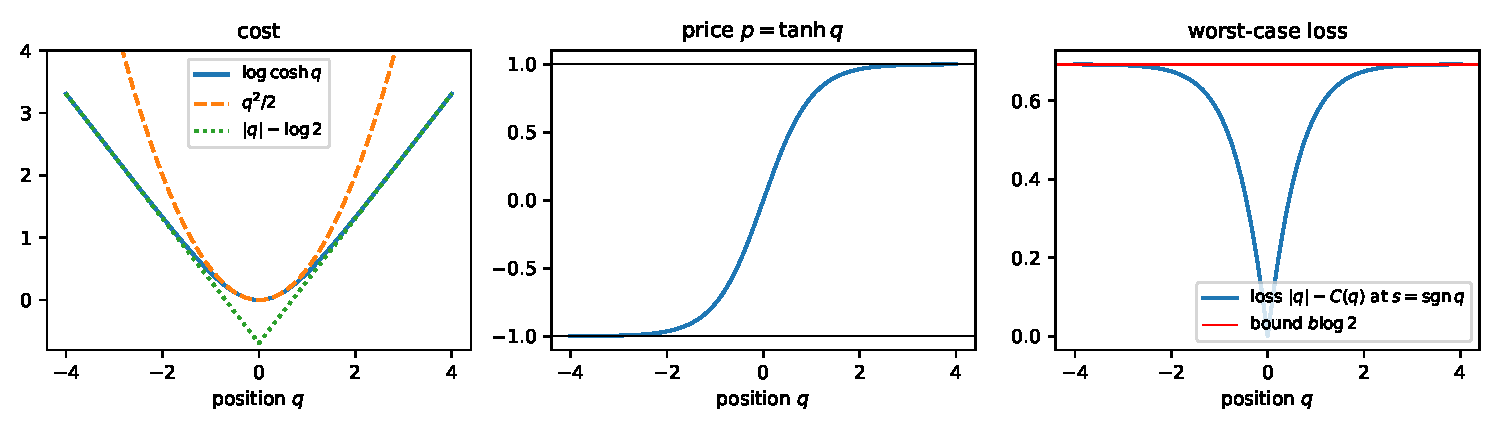
\includegraphics[width=\textwidth]{figures/fig1_one_contract.pdf}
\caption{One contract, $b=1$. Left: cost $C(q)=\log\cosh q$ against the quadratic $q^2/2$ and the asymptote
$|q|-\log2$. Middle: price $p(q)=\tanh q$, saturating at $\pm1$. Right: the realised loss $|q|-C(q)$ against the
worst settlement $s=\sgn q$, which approaches but never exceeds the exact bound $\log 2$ (Theorem~\ref{thm:loss}).}
\label{fig:one}
\end{figure}

\begin{figure}[t]
\centering
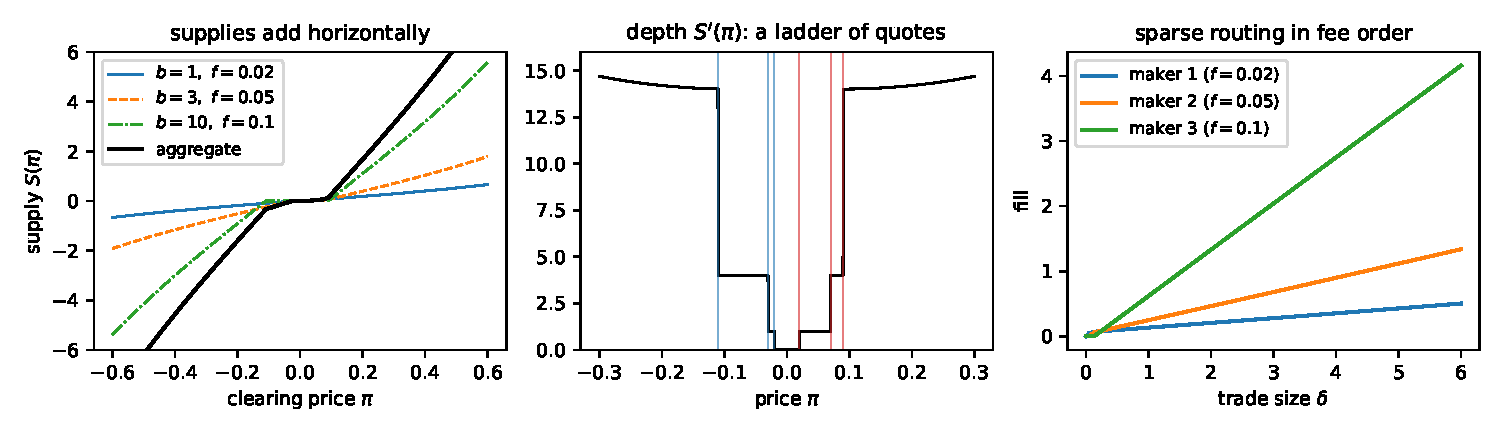
\includegraphics[width=\textwidth]{figures/fig2_book.pdf}
\caption{Three makers on one contract, with capital, fee and current price $(b_k,f_k,p_k)$ equal to $(1,0.02,0)$,
$(3,0.05,0.02)$ and $(10,0.10,-0.01)$. Left: each
maker's supply \eqref{eq:supply1d} is zero inside its own band and the aggregate is their horizontal sum
(Theorem~\ref{thm:book}). Middle: the depth $S'(\pi)$ near the quotes is a ladder with a rung at every bid (blue) and ask (red); this is the
consolidated book. Right: the fill allocation of a trade of size $\delta$ across the three makers: small trades go
entirely to the cheapest maker and larger trades eat through the others in fee order, with exact zeros.}
\label{fig:book}
\end{figure}

\begin{figure}[t]
\centering
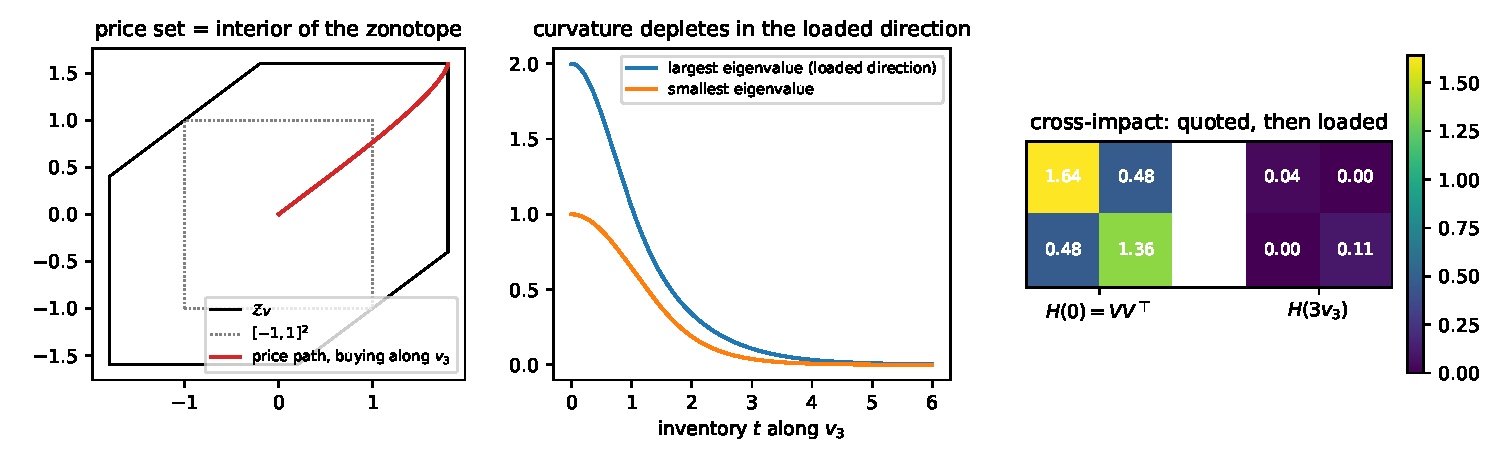
\includegraphics[width=\textwidth]{figures/fig3_curvature.pdf}
\caption{Two contracts, $V=[v_1\,v_2\,v_3]$ with $v_1=e_1,\ v_2=e_2,\ v_3=(0.8,0.6)$, $b=1$. Left: the zonotope
$\zono_V=V[-1,1]^3$ (the price set and the set of settlements with finite worst-case loss) with the price path of a
trader buying along $v_3$. Middle: the eigenvalues of the Hessian $H(q)$ along that path; the loaded direction
flattens as $\sech^2$ falls while the orthogonal direction keeps its curvature. Right: the cross-impact matrix at the
origin (the quoted covariance $VV^{\top}$) and after loading.}
\label{fig:curv}
\end{figure}

\section{Related work}\label{sec:related}

Cost-function market makers originate with Hanson's market scoring rules \citep{hanson2003,hanson2007}; the
utility-based view is \citet{chen2007utility}; the convex-analytic framework, including the characterisation of
bounded loss through the conjugate and the identification of price dynamics with follow-the-regularised-leader, is
\citet{abernethy2013}. The scalar fee--spread duality, the exact no-trade interval for non-convex costs, and the order book as the
horizontal sum of fee-shifted supplies are developed in \citet{cotton2026nonconvex}. The many-contract form and the
closed-form family extend them. Liquidity-sensitive and profit-charging variants of LMSR are studied by
\citet{othman2013}; our fee differs in that it is per unit and $\ell_1$, which produces exact sparsity and a dead
band rather than a continuously widening spread.

Bounded settlements of the $\tanh$ form are standard in
robust statistics as bounded-influence transforms \citep{huber1981}. The dead-band view of the spread is the
adverse-selection view of \citet{glosten1985}; inventory-based spreads in the style of \citet{avellaneda2008} are
complementary and can be read off the Hessian in Section~\ref{sec:curvature}.

Inf-convolution and the additivity
of conjugates are classical \citep{rockafellar1970}; their use for aggregating supply is Marshall's, and the
multiproduct cost reading is \citet{baumol1982}. Constant-function market makers in decentralised finance
\citep{angeris2020} are also convex-duality objects (trading sets and their support functions), and their
aggregation across pools by routing \citep{angeris2022} is an inf-convolution of the same kind, though without
the fee-as-band structure and with reserves in place of a loss bound.

Economic-derivatives auctions on
macroeconomic releases \citep{gurkaynak2005} are the closest historical precedent for markets on standardised
surprises; they were episodic parimutuel auctions without shared-state makers. The identification of market
selection with Bayesian averaging is \citet{blume1992}; cost-function makers as online learners is
\citet{chen2010}.

\section{Conclusion}

A market maker that posts two numbers, a fee and a capital, and optionally a few residual vectors, has stated a
bounded loss exactly, quoted a covariance it accepts fills under, and set its own spread; a set of such makers aggregates, by
convex duality alone, into a consolidated limit order book with sparse routing and additive liquidity. The
protocol needs to fix only the settlement rule. Open questions remain about the dynamics: the lifecycle of such
markets as the baseline freezes and the observation approaches, the toxicity of near-settlement flow, and the
equilibrium fees that a population of competing makers settles on. Those are empirical questions.

\bibliographystyle{plainnat}
\bibliography{refs}

\appendix
\section{Numerical verification}\label{app:verify}

The script \texttt{verify.py}, distributed with the source, checks the following with the stated tolerances and
prints a pass/fail line for each; all pass.
\begin{enumerate}[leftmargin=2em,itemsep=1pt]
\item \textbf{Conjugate formula} (Lemma~\ref{lem:conj}). For $V=I_3$, $b\in\{0.5,1,3\}$ and 200 random $s\in(-1,1)^3$,
$\sup_q\{\ip{q}{s}-C(q)\}$ by numerical maximisation agrees with $b\sum_i\lcs(s_i)$ to $10^{-6}$. For a non-square
$V$ ($n=2$, $D=3$) the numerical supremum agrees with the constrained minimum in \eqref{eq:conj} to $10^{-5}$.

\item \textbf{Loss bound and attainment} (Theorem~\ref{thm:loss}). For 2000 random trade sequences and every vertex
settlement, loss $\le b\,D\log2+10^{-9}$; along $q_t=tV(V^{\top}V)^{-1}y$ the loss exceeds $b\,D\log2-10^{-6}$ for
large $t$. For a settlement outside $\zono_V$ the loss along a ray grows linearly.

\item \textbf{Price set} (Proposition~\ref{prop:priceset}). For $D=n$ and random $q$, $V^{-1}p(q)\in(-1,1)^{n}$, and
$q(p(q))=q$ to $10^{-9}$.

\item \textbf{Dead band} (Proposition~\ref{prop:band}). For random $q,\pi,f$ the maximiser of
$\ip{\delta}{\pi}-C^{f}_{q}(\delta)$ (found by a proximal-gradient iteration to $10^{-10}$) is zero iff
$\|\pi-p(q)\|_\infty\le f$, and the active-set conditions of item 2 hold to $10^{-7}$.

\item \textbf{Conjugates add} (Theorem~\ref{thm:book}(1)). For two one-dimensional fee-bearing makers, the conjugate
of the inf-convolution computed by brute force on a grid equals the sum of the conjugates to $10^{-4}$ (the grid resolution).

\item \textbf{One clearing price and horizontal summation} (Theorem~\ref{thm:book}(2,3,5)). For three makers and 200
random trade sizes, the optimal split found by direct minimisation agrees with the bisection on
\eqref{eq:supply1d} to $10^{-7}$ in each fill; inactive makers have fills exactly zero; the Lagrange multiplier equals
the clearing price.

\item \textbf{Liquidity adds} (Theorem~\ref{thm:book}(4)). For three fee-free makers at the origin the numerical
Hessian of the inf-convolution at $0$ has inverse equal to $\sum_kH_k(0)^{-1}$ to $10^{-5}$.

\item \textbf{Bregman identity} (equation~\eqref{eq:bregman}) to $10^{-9}$ for random $q,s$.

\item \textbf{Re-centring} (Proposition~\ref{prop:conservation}). A maker re-centred $m$ times attains loss within
$10^{-4}$ of $(m+1)b\log2$ in one dimension.
\end{enumerate}

\end{document}
